\pdfminorversion=4
\documentclass[]{beamer}
\mode<presentation>
% Time-stamp: <2021-07-10 14:40:04 (jonahm)>

% beamer stuff
% Gives us the bottom line with all the goodies
\useoutertheme{infolines}
% Just the theme to use. Should be built into bemaer. Setting the
% height gets rid of a whole lot of whitespace
\usetheme[height=7mm]{Rochester}
\usefonttheme{serif}
% Usually beamer gives you navigation hyperlinks on the bottom
% right. I turned this off. It's annoying.
\setbeamertemplate{navigation symbols}{} 
% Makes my text boxes look pretty
\setbeamertemplate{blocks}[rounded][shadow=true] 
% Makes my bullet points 3d balls
\setbeamertemplate{items}[ball]

% Josh's packages
\usepackage{multimedia}
\usepackage{graphicx}

% Packages for me
\usepackage{amsmath,amssymb,latexsym,amsthm}
\usepackage[mathscr]{eucal}
\usepackage{mathrsfs}
\usepackage{verbatim}
\usepackage{braket}
\usepackage{listings}
\usepackage{xcolor}
% \usepackage[usenames,dvipsnames,svgnames,table]{xcolor}
\usepackage{fancybox}
\usepackage{animate}
% \usepackage{media9}
\usepackage{multicol}
\usepackage{mdframed}
\usepackage{hyperref}
%\usepackage{scalerel}
\usepackage[outline]{contour}
\contourlength{1.2pt}

% Macros

%Blackboard Bold
\newcommand{\R}{\mathbb{R}}
\newcommand{\Z}{\mathbb{Z}}
\newcommand{\N}{\mathbb{N}}
\newcommand{\Q}{\mathbb{Q}}
\newcommand{\A}{\mathbb{A}}
\newcommand{\E}{\mathbb{E}}
% other
\newcommand{\eval}{\biggr\rvert} %evaluated at
\newcommand{\myvec}[1]{\mathbf{#1}} % vectors for me
% total derivatives 
\newcommand{\diff}[2]{\frac{d #1}{d #2}} 
\newcommand{\dd}[1]{\frac{d}{d #1}}
% partial derivatives
\newcommand{\pd}[2]{\frac{\partial #1}{\partial #2}} 
\newcommand{\pdd}[1]{\frac{\partial}{\partial #1}} 
% Order operator
\DeclareRobustCommand{\orderof}{\ensuremath{\mathcal{O}}}

% braces
\newcommand{\paren}[1]{\left( #1 \right)}
\newcommand{\sqrbrace}[1]{\left[ #1 \right]}
\newcommand{\curlybrace}[1]{\left\{ #1 \right\}}
\newcommand{\inner}[1]{\paren{#1}}
\newcommand{\norm}[1]{\left| #1 \right|_2}

% g
\newcommand{\detg}{\sqrt{-g}}

% neutrinos
\newcommand{\eepsilon}{\epsilon} % energy
\newcommand{\fin}{f\in \{\nu_e,\nu_{\bar{e}},\nu_x\}}
\newcommand{\sign}{\text{sign}(f)}
\newcommand{\jnuf}{j_{\eepsilon,f}}
\newcommand{\etanuf}{\eta_{\eepsilon,f}}
\newcommand{\Inuf}{I_{\eepsilon,f}}
\newcommand{\chinuf}{\chi_{\eepsilon,f}}
\newcommand{\sigmanuf}{\sigma_{\eepsilon,f}}
\newcommand{\alphanuf}{\alpha_{\eepsilon,f}}
\newcommand{\numin}{\nu_{\text{min}}}
\newcommand{\numax}{\nu_{\text{max}}}


% tikz
\usepackage{tikz}
\usepackage{pgfplots}
\usetikzlibrary{arrows}
\usetikzlibrary{decorations.pathmorphing}
\usetikzlibrary{decorations.markings}
\usetikzlibrary{arrows.meta,bending}
% From texzample periodic table
% \usepackage[active,tightpage]{preview}
\usetikzlibrary{shapes,calc}

% Keys to support piece-wise uncovering of elements in TikZ pictures:
% \node[visible on=<2->](foo){Foo}
% \node[visible on=<{2,4}>](bar){Bar}   % put braces around comma expressions
% 
% Internally works by setting opacity=0 when invisible, which has the 
% adavantage (compared to \node<2->(foo){Foo} that the node is always there, hence
% always consumes space plus that coordinate (foo) is always available.
% 
% The actual command that implements the invisibility can be overriden
% by altering the style invisible. For instance \tikzsset{invisible/.style={opacity=0.2}}
% would dim the "invisible" parts. Alternatively, the color might be set to white, if the
% output driver does not support transparencies (e.g., PS) 
% 
\tikzset{
  invisible/.style={opacity=0},
  visible on/.style={alt={#1{}{invisible}}},
  alt/.code args={<#1>#2#3}{%
    \alt<#1>{\pgfkeysalso{#2}}{\pgfkeysalso{#3}} % \pgfkeysalso doesn't change the path
  },
}

% some nice flowchart features
\tikzset{
    mynode/.style={rectangle,rounded corners,draw=black, top color=white, bottom color=yellow!50,very thick, inner sep=1em, minimum size=3em, text centered},
    myarrow/.style={->, >=latex', shorten >=1pt, thick},
    mylabel/.style={text width=7em, text centered} 
}  

% squigly arrow
\tikzset{zigzag it/.style={decorate, decoration=zigzag}}

% Color morphing arrow
\tikzset{colormorph/.style n args={3}{
    postaction={
    decorate,
    decoration={
    markings,
    mark=between positions 0 and \pgfdecoratedpathlength step 0.5pt with {
    \pgfmathsetmacro\myval{multiply(
        divide(
        \pgfkeysvalueof{/pgf/decoration/mark info/distance from start}, \pgfdecoratedpathlength
        ),
        100
    )};
    \pgfsetfillcolor{#3!\myval!#2};
    \pgfpathcircle{\pgfpointorigin}{#1};
    \pgfusepath{fill};}
}}}}

\newcommand{\CommonElementTextFormat}[4]
{
  \begin{minipage}{2.2cm}
    \centering
      {\textbf{#1} \hfill #2}%
      \linebreak \linebreak
      {\textbf{#3}}%
      \linebreak \linebreak
      {{#4}}
  \end{minipage}
}

\newcommand{\NaturalElementTextFormat}[4]
{
  \CommonElementTextFormat{#1}{#2}{\LARGE {#3}}{#4}
}

\newcommand{\OutlineText}[1]
{
  % Couldn't find a nicer way of doing an outline font with TikZ
  % other than using pdfliteral 1 Tr
  %
  \pdfliteral direct {0.5 w 1 Tr}{#1}%
  \pdfliteral direct {1 w 0 Tr}%
}

\newcommand{\SyntheticElementTextFormat}[4]
{
  \CommonElementTextFormat{#1}{#2}{\OutlineText{\LARGE #3}}{#4}
}

% define a really nice visible "purple"
\definecolor{gimppurple}{HTML}{AD26FB}
% a light grey
\definecolor{lightgrey}{HTML}{E0E0E0}
% for highlighting
\definecolor{deepblue}{rgb}{0,0,0.5}
\definecolor{deepred}{rgb}{0.6,0,0}
\definecolor{deepgreen}{rgb}{0,0.5,0}

% fonts
% Default fixed font does not support bold face
\DeclareFixedFont{\ttb}{T1}{txtt}{bx}{n}{12} % for bold
\DeclareFixedFont{\ttm}{T1}{txtt}{m}{n}{12}  % for normal

% Python style for highlighting
\newcommand\pythonstyle{\lstset{
language=Python,
basicstyle=\ttm,
otherkeywords={self},
keywordstyle=\ttb\color{deepblue},
emph={__init__},           
emphstyle=\ttb\color{deepred},
commentstyle=\ttfamily\color{deepred},
stringstyle=\color{deepgreen},
frame=tb,                     
showstringspaces=false        
}}

% Python environment
\lstnewenvironment{python}[1][]
{
\pythonstyle
\lstset{#1}
}
{}

\newcommand{\backupbegin}{
   \newcounter{finalframe}
   \setcounter{finalframe}{\value{framenumber}}
}
\newcommand{\backupend}{
   \setcounter{framenumber}{\value{finalframe}}
}

% Automatically generates section breaker slides
\AtBeginSection[]{
  \begin{frame}[plain]
  \vfill
  \centering
  \begin{beamercolorbox}[sep=8pt,center,shadow=true,rounded=true]{title}
    \usebeamerfont{title}\insertsectionhead\par%
  \end{beamercolorbox}
  \vfill
  \end{frame}
}

\title[Fusion in Space]{Fusion in Space: Nuclear Astrophysics, Neutron Star Mergers, and Accretion Disks}
% \subtitle{Models and Implications}
\author[J. Miller]{\textcolor{blue}{Jonah M. Miller}}
\institute[LANL]{Los Alamos National Laboratory}
% \titlegraphic{\vspace{1cm}}
% \titlegraphic{\includegraphics[height=0.25\textheight]{3d_render}}
\date[CRLC]{SHI CRLC Virtual Seminar}

\graphicspath{{figures/}}

\begin{document}

\begin{frame}[plain]
    \tikz [remember picture, overlay] 
    \node at ([xshift=2cm,yshift=-2cm]current page.west)
    {\includegraphics[width=0.25\textwidth,clip,trim={150 0 150 0}]{3d_render}};
    \tikz [remember picture, overlay] 
    \node at ([xshift=-2cm,yshift=-2cm]current page.east)
    {\includegraphics[width=0.25\textwidth,clip,trim={0 0 0 0}]{visit0006-gimp3}};
  \titlepage
\end{frame}

\begin{frame}
  \frametitle{A Deceptively Simple Question}
  \begin{itemize}
  \item Where does stuff come from?
  \end{itemize}
  \resizebox{12cm}{!}{
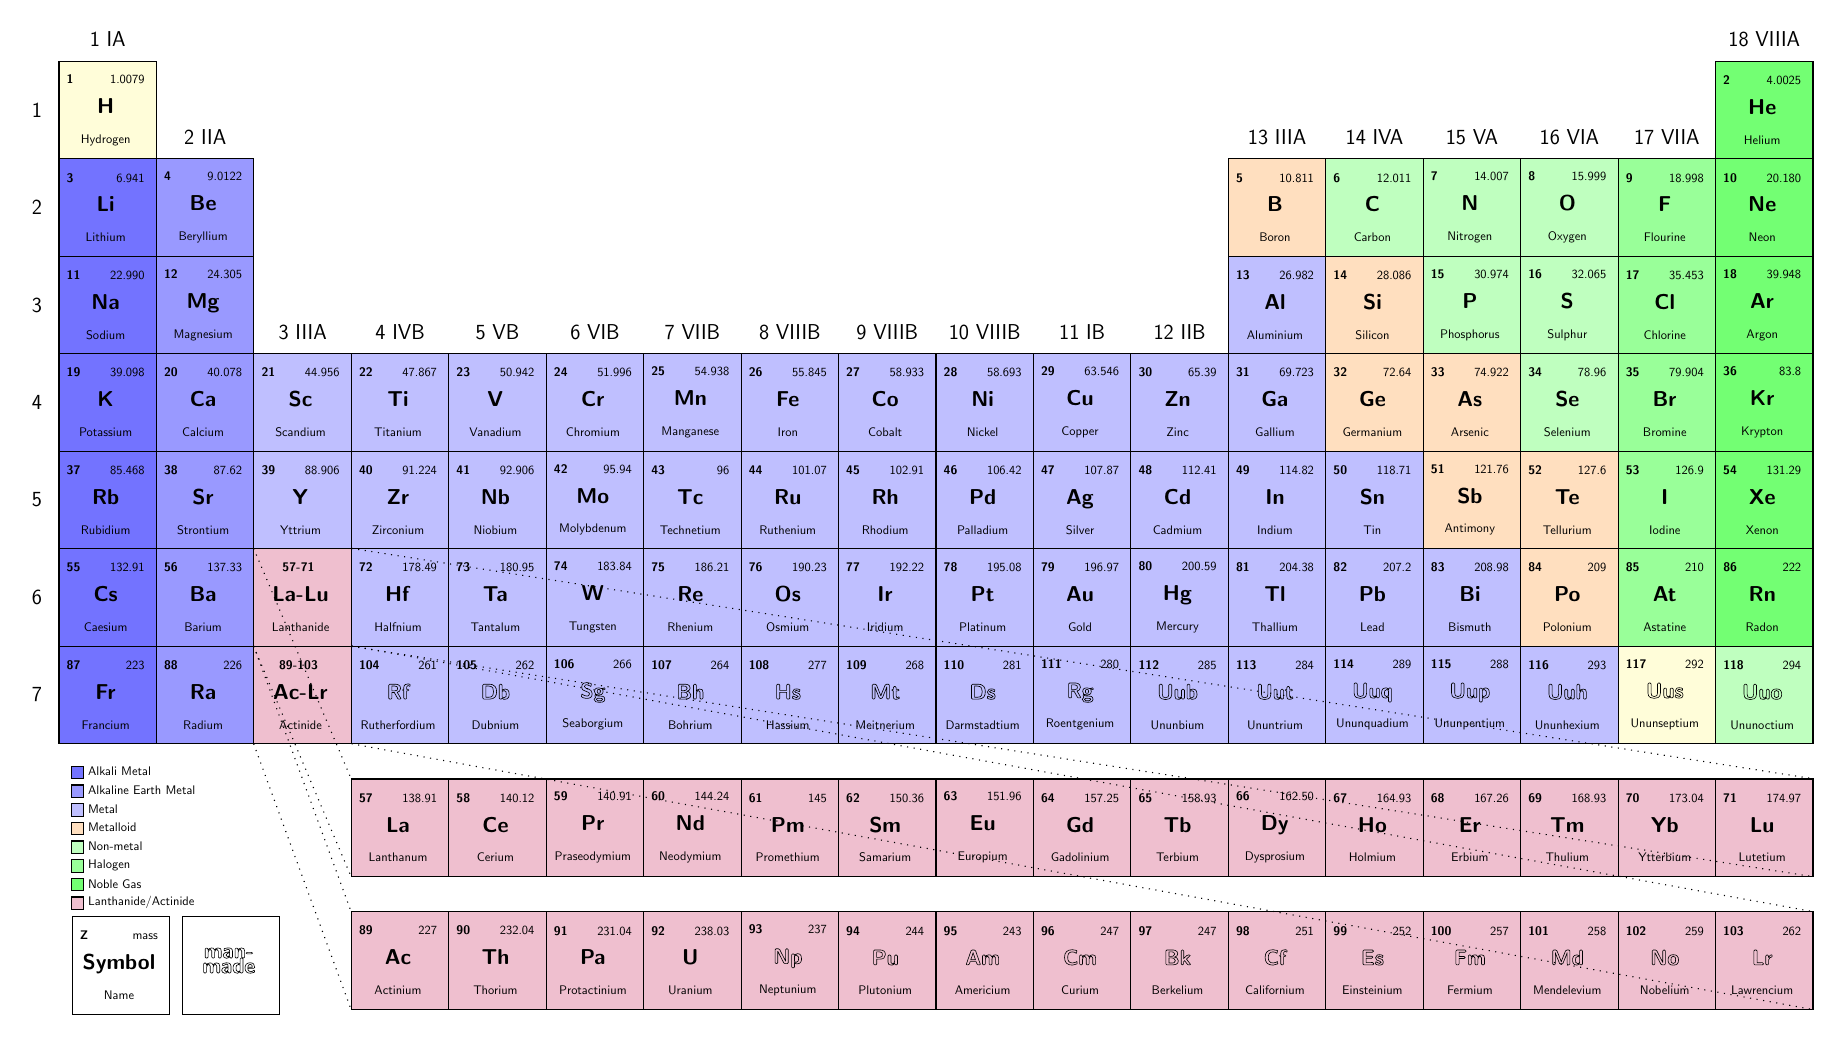
\begin{tikzpicture}[font=\sffamily, scale=0.45, transform shape]

%% Fill Color Styles
  \tikzstyle{ElementFill} = [fill=yellow!15]
  \tikzstyle{AlkaliMetalFill} = [fill=blue!55]
  \tikzstyle{AlkalineEarthMetalFill} = [fill=blue!40]
  \tikzstyle{MetalFill} = [fill=blue!25]
  \tikzstyle{MetalloidFill} = [fill=orange!25]
  \tikzstyle{NonmetalFill} = [fill=green!25]
  \tikzstyle{HalogenFill} = [fill=green!40]
  \tikzstyle{NobleGasFill} = [fill=green!55]
  \tikzstyle{LanthanideActinideFill} = [fill=purple!25]

%% Element Styles
  \tikzstyle{Element} = [draw=black, ElementFill,
    minimum width=2.75cm, minimum height=2.75cm, node distance=2.75cm]
  \tikzstyle{AlkaliMetal} = [Element, AlkaliMetalFill]
  \tikzstyle{AlkalineEarthMetal} = [Element, AlkalineEarthMetalFill]
  \tikzstyle{Metal} = [Element, MetalFill]
  \tikzstyle{Metalloid} = [Element, MetalloidFill]
  \tikzstyle{Nonmetal} = [Element, NonmetalFill]
  \tikzstyle{Halogen} = [Element, HalogenFill]
  \tikzstyle{NobleGas} = [Element, NobleGasFill]
  \tikzstyle{LanthanideActinide} = [Element, LanthanideActinideFill]
  \tikzstyle{PeriodLabel} = [font={\sffamily\LARGE}, node distance=2.0cm]
  \tikzstyle{GroupLabel} = [font={\sffamily\LARGE}, minimum width=2.75cm, node distance=2.0cm]
  \tikzstyle{TitleLabel} = [font={\sffamily\Huge\bfseries}]

%% Group 1 - IA
  \node[name=H, Element] {\NaturalElementTextFormat{1}{1.0079}{H}{Hydrogen}};
  \node[name=Li, below of=H, AlkaliMetal] {\NaturalElementTextFormat{3}{6.941}{Li}{Lithium}};
  \node[name=Na, below of=Li, AlkaliMetal] {\NaturalElementTextFormat{11}{22.990}{Na}{Sodium}};
  \node[name=K, below of=Na, AlkaliMetal] {\NaturalElementTextFormat{19}{39.098}{K}{Potassium}};
  \node[name=Rb, below of=K, AlkaliMetal] {\NaturalElementTextFormat{37}{85.468}{Rb}{Rubidium}};
  \node[name=Cs, below of=Rb, AlkaliMetal] {\NaturalElementTextFormat{55}{132.91}{Cs}{Caesium}};
  \node[name=Fr, below of=Cs, AlkaliMetal] {\NaturalElementTextFormat{87}{223}{Fr}{Francium}};

%% Group 2 - IIA
  \node[name=Be, right of=Li, AlkalineEarthMetal] {\NaturalElementTextFormat{4}{9.0122}{Be}{Beryllium}};
  \node[name=Mg, below of=Be, AlkalineEarthMetal] {\NaturalElementTextFormat{12}{24.305}{Mg}{Magnesium}};
  \node[name=Ca, below of=Mg, AlkalineEarthMetal] {\NaturalElementTextFormat{20}{40.078}{Ca}{Calcium}};
  \node[name=Sr, below of=Ca, AlkalineEarthMetal] {\NaturalElementTextFormat{38}{87.62}{Sr}{Strontium}};
  \node[name=Ba, below of=Sr, AlkalineEarthMetal] {\NaturalElementTextFormat{56}{137.33}{Ba}{Barium}};
  \node[name=Ra, below of=Ba, AlkalineEarthMetal] {\NaturalElementTextFormat{88}{226}{Ra}{Radium}};

%% Group 3 - IIIB
  \node[name=Sc, right of=Ca, Metal] {\NaturalElementTextFormat{21}{44.956}{Sc}{Scandium}};
  \node[name=Y, below of=Sc, Metal] {\NaturalElementTextFormat{39}{88.906}{Y}{Yttrium}};
  \node[name=LaLu, below of=Y, LanthanideActinide] {\NaturalElementTextFormat{57-71}{}{La-Lu}{Lanthanide}};
  \node[name=AcLr, below of=LaLu, LanthanideActinide] {\NaturalElementTextFormat{89-103}{}{Ac-Lr}{Actinide}};

%% Group 4 - IVB
  \node[name=Ti, right of=Sc, Metal] {\NaturalElementTextFormat{22}{47.867}{Ti}{Titanium}};
  \node[name=Zr, below of=Ti, Metal] {\NaturalElementTextFormat{40}{91.224}{Zr}{Zirconium}};
  \node[name=Hf, below of=Zr, Metal] {\NaturalElementTextFormat{72}{178.49}{Hf}{Halfnium}};
  \node[name=Rf, below of=Hf, Metal] {\SyntheticElementTextFormat{104}{261}{Rf}{Rutherfordium}};

%% Group 5 - VB
  \node[name=V, right of=Ti, Metal] {\NaturalElementTextFormat{23}{50.942}{V}{Vanadium}};
  \node[name=Nb, below of=V, Metal] {\NaturalElementTextFormat{41}{92.906}{Nb}{Niobium}};
  \node[name=Ta, below of=Nb, Metal] {\NaturalElementTextFormat{73}{180.95}{Ta}{Tantalum}};
  \node[name=Db, below of=Ta, Metal] {\SyntheticElementTextFormat{105}{262}{Db}{Dubnium}};

%% Group 6 - VIB
  \node[name=Cr, right of=V, Metal] {\NaturalElementTextFormat{24}{51.996}{Cr}{Chromium}};
  \node[name=Mo, below of=Cr, Metal] {\NaturalElementTextFormat{42}{95.94}{Mo}{Molybdenum}};
  \node[name=W, below of=Mo, Metal] {\NaturalElementTextFormat{74}{183.84}{W}{Tungsten}};
  \node[name=Sg, below of=W, Metal] {\SyntheticElementTextFormat{106}{266}{Sg}{Seaborgium}};

%% Group 7 - VIIB
  \node[name=Mn, right of=Cr, Metal] {\NaturalElementTextFormat{25}{54.938}{Mn}{Manganese}};
  \node[name=Tc, below of=Mn, Metal] {\NaturalElementTextFormat{43}{96}{Tc}{Technetium}};
  \node[name=Re, below of=Tc, Metal] {\NaturalElementTextFormat{75}{186.21}{Re}{Rhenium}};
  \node[name=Bh, below of=Re, Metal] {\SyntheticElementTextFormat{107}{264}{Bh}{Bohrium}};

%% Group 8 - VIIIB
  \node[name=Fe, right of=Mn, Metal] {\NaturalElementTextFormat{26}{55.845}{Fe}{Iron}};
  \node[name=Ru, below of=Fe, Metal] {\NaturalElementTextFormat{44}{101.07}{Ru}{Ruthenium}};
  \node[name=Os, below of=Ru, Metal] {\NaturalElementTextFormat{76}{190.23}{Os}{Osmium}};
  \node[name=Hs, below of=Os, Metal] {\SyntheticElementTextFormat{108}{277}{Hs}{Hassium}};

%% Group 9 - VIIIB
  \node[name=Co, right of=Fe, Metal] {\NaturalElementTextFormat{27}{58.933}{Co}{Cobalt}};
  \node[name=Rh, below of=Co, Metal] {\NaturalElementTextFormat{45}{102.91}{Rh}{Rhodium}};
  \node[name=Ir, below of=Rh, Metal] {\NaturalElementTextFormat{77}{192.22}{Ir}{Iridium}};
  \node[name=Mt, below of=Ir, Metal] {\SyntheticElementTextFormat{109}{268}{Mt}{Meitnerium}};

%% Group 10 - VIIIB
  \node[name=Ni, right of=Co, Metal] {\NaturalElementTextFormat{28}{58.693}{Ni}{Nickel}};
  \node[name=Pd, below of=Ni, Metal] {\NaturalElementTextFormat{46}{106.42}{Pd}{Palladium}};
  \node[name=Pt, below of=Pd, Metal] {\NaturalElementTextFormat{78}{195.08}{Pt}{Platinum}};
  \node[name=Ds, below of=Pt, Metal] {\SyntheticElementTextFormat{110}{281}{Ds}{Darmstadtium}};

%% Group 11 - IB
  \node[name=Cu, right of=Ni, Metal] {\NaturalElementTextFormat{29}{63.546}{Cu}{Copper}};
  \node[name=Ag, below of=Cu, Metal] {\NaturalElementTextFormat{47}{107.87}{Ag}{Silver}};
  \node[name=Au, below of=Ag, Metal] {\NaturalElementTextFormat{79}{196.97}{Au}{Gold}};
  \node[name=Rg, below of=Au, Metal] {\SyntheticElementTextFormat{111}{280}{Rg}{Roentgenium}};

%% Group 12 - IIB
  \node[name=Zn, right of=Cu, Metal] {\NaturalElementTextFormat{30}{65.39}{Zn}{Zinc}};
  \node[name=Cd, below of=Zn, Metal] {\NaturalElementTextFormat{48}{112.41}{Cd}{Cadmium}};
  \node[name=Hg, below of=Cd, Metal] {\NaturalElementTextFormat{80}{200.59}{Hg}{Mercury}};
  \node[name=Uub, below of=Hg, Metal] {\SyntheticElementTextFormat{112}{285}{Uub}{Ununbium}};

%% Group 13 - IIIA
  \node[name=Ga, right of=Zn, Metal] {\NaturalElementTextFormat{31}{69.723}{Ga}{Gallium}};
  \node[name=Al, above of=Ga, Metal] {\NaturalElementTextFormat{13}{26.982}{Al}{Aluminium}};
  \node[name=B, above of=Al, Metalloid] {\NaturalElementTextFormat{5}{10.811}{B}{Boron}};
  \node[name=In, below of=Ga, Metal] {\NaturalElementTextFormat{49}{114.82}{In}{Indium}};
  \node[name=Tl, below of=In, Metal] {\NaturalElementTextFormat{81}{204.38}{Tl}{Thallium}};
  \node[name=Uut, below of=Tl, Metal] {\SyntheticElementTextFormat{113}{284}{Uut}{Ununtrium}};

%% Group 14 - IVA
  \node[name=C, right of=B, Nonmetal] {\NaturalElementTextFormat{6}{12.011}{C}{Carbon}};
  \node[name=Si, below of=C, Metalloid] {\NaturalElementTextFormat{14}{28.086}{Si}{Silicon}};
  \node[name=Ge, below of=Si, Metalloid] {\NaturalElementTextFormat{32}{72.64}{Ge}{Germanium}};
  \node[name=Sn, below of=Ge, Metal] {\NaturalElementTextFormat{50}{118.71}{Sn}{Tin}};
  \node[name=Pb, below of=Sn, Metal] {\NaturalElementTextFormat{82}{207.2}{Pb}{Lead}};
  \node[name=Uuq, below of=Pb, Metal] {\SyntheticElementTextFormat{114}{289}{Uuq}{Ununquadium}};

%% Group 15 - VA
  \node[name=N, right of=C, Nonmetal] {\NaturalElementTextFormat{7}{14.007}{N}{Nitrogen}};
  \node[name=P, below of=N, Nonmetal] {\NaturalElementTextFormat{15}{30.974}{P}{Phosphorus}};
  \node[name=As, below of=P, Metalloid] {\NaturalElementTextFormat{33}{74.922}{As}{Arsenic}};
  \node[name=Sb, below of=As, Metalloid] {\NaturalElementTextFormat{51}{121.76}{Sb}{Antimony}};
  \node[name=Bi, below of=Sb, Metal] {\NaturalElementTextFormat{83}{208.98}{Bi}{Bismuth}};
  \node[name=Uup, below of=Bi, Metal] {\SyntheticElementTextFormat{115}{288}{Uup}{Ununpentium}};

%% Group 16 - VIA
  \node[name=O, right of=N, Nonmetal] {\NaturalElementTextFormat{8}{15.999}{O}{Oxygen}};
  \node[name=S, below of=O, Nonmetal] {\NaturalElementTextFormat{16}{32.065}{S}{Sulphur}};
  \node[name=Se, below of=S, Nonmetal] {\NaturalElementTextFormat{34}{78.96}{Se}{Selenium}};
  \node[name=Te, below of=Se, Metalloid] {\NaturalElementTextFormat{52}{127.6}{Te}{Tellurium}};
  \node[name=Po, below of=Te, Metalloid] {\NaturalElementTextFormat{84}{209}{Po}{Polonium}};
  \node[name=Uuh, below of=Po, Metal] {\SyntheticElementTextFormat{116}{293}{Uuh}{Ununhexium}};

%% Group 17 - VIIA
  \node[name=F, right of=O, Halogen] {\NaturalElementTextFormat{9}{18.998}{F}{Flourine}};
  \node[name=Cl, below of=F, Halogen] {\NaturalElementTextFormat{17}{35.453}{Cl}{Chlorine}};
  \node[name=Br, below of=Cl, Halogen] {\NaturalElementTextFormat{35}{79.904}{Br}{Bromine}};
  \node[name=I, below of=Br, Halogen] {\NaturalElementTextFormat{53}{126.9}{I}{Iodine}};
  \node[name=At, below of=I, Halogen] {\NaturalElementTextFormat{85}{210}{At}{Astatine}};
  \node[name=Uus, below of=At, Element] {\SyntheticElementTextFormat{117}{292}{Uus}{Ununseptium}}; 

%% Group 18 - VIIIA
  \node[name=Ne, right of=F, NobleGas] {\NaturalElementTextFormat{10}{20.180}{Ne}{Neon}};
  \node[name=He, above of=Ne, NobleGas] {\NaturalElementTextFormat{2}{4.0025}{He}{Helium}};
  \node[name=Ar, below of=Ne, NobleGas] {\NaturalElementTextFormat{18}{39.948}{Ar}{Argon}};
  \node[name=Kr, below of=Ar, NobleGas] {\NaturalElementTextFormat{36}{83.8}{Kr}{Krypton}};
  \node[name=Xe, below of=Kr, NobleGas] {\NaturalElementTextFormat{54}{131.29}{Xe}{Xenon}};
  \node[name=Rn, below of=Xe, NobleGas] {\NaturalElementTextFormat{86}{222}{Rn}{Radon}};
  \node[name=Uuo, below of=Rn, Nonmetal] {\SyntheticElementTextFormat{118}{294}{Uuo}{Ununoctium}}; 

%% Period
  \node[name=Period1, left of=H, PeriodLabel] {1};
  \node[name=Period2, left of=Li, PeriodLabel] {2};
  \node[name=Period3, left of=Na, PeriodLabel] {3}; 
  \node[name=Period4, left of=K, PeriodLabel] {4}; 
  \node[name=Period5, left of=Rb, PeriodLabel] {5};
  \node[name=Period6, left of=Cs, PeriodLabel] {6};
  \node[name=Period7, left of=Fr, PeriodLabel] {7};

%% Group
  \node[name=Group1, above of=H, GroupLabel] {1 \hfill IA};
  \node[name=Group2, above of=Be, GroupLabel] {2 \hfill IIA};
  \node[name=Group3, above of=Sc, GroupLabel] {3 \hfill IIIA};
  \node[name=Group4, above of=Ti, GroupLabel] {4 \hfill IVB};
  \node[name=Group5, above of=V, GroupLabel] {5 \hfill VB};
  \node[name=Group6, above of=Cr, GroupLabel] {6 \hfill VIB};
  \node[name=Group7, above of=Mn, GroupLabel] {7 \hfill VIIB};
  \node[name=Group8, above of=Fe, GroupLabel] {8 \hfill VIIIB};
  \node[name=Group9, above of=Co, GroupLabel] {9 \hfill VIIIB};
  \node[name=Group10, above of=Ni, GroupLabel] {10 \hfill VIIIB};
  \node[name=Group11, above of=Cu, GroupLabel] {11 \hfill IB};
  \node[name=Group12, above of=Zn, GroupLabel] {12 \hfill IIB};
  \node[name=Group13, above of=B, GroupLabel] {13 \hfill IIIA};
  \node[name=Group14, above of=C, GroupLabel] {14 \hfill IVA};
  \node[name=Group15, above of=N, GroupLabel] {15 \hfill VA};
  \node[name=Group16, above of=O, GroupLabel] {16 \hfill VIA};
  \node[name=Group17, above of=F, GroupLabel] {17 \hfill VIIA};
  \node[name=Group18, above of=He, GroupLabel] {18 \hfill VIIIA};

%% Lanthanide
  \node[name=La, below of=Rf, LanthanideActinide, yshift=-1cm] {\NaturalElementTextFormat{57}{138.91}{La}{Lanthanum}};
  \node[name=Ce, right of=La, LanthanideActinide] {\NaturalElementTextFormat{58}{140.12}{Ce}{Cerium}};
  \node[name=Pr, right of=Ce, LanthanideActinide] {\NaturalElementTextFormat{59}{140.91}{Pr}{Praseodymium}};
  \node[name=Nd, right of=Pr, LanthanideActinide] {\NaturalElementTextFormat{60}{144.24}{Nd}{Neodymium}};
  \node[name=Pm, right of=Nd, LanthanideActinide] {\NaturalElementTextFormat{61}{145}{Pm}{Promethium}};
  \node[name=Sm, right of=Pm, LanthanideActinide] {\NaturalElementTextFormat{62}{150.36}{Sm}{Samarium}};
  \node[name=Eu, right of=Sm, LanthanideActinide] {\NaturalElementTextFormat{63}{151.96}{Eu}{Europium}};
  \node[name=Gd, right of=Eu, LanthanideActinide] {\NaturalElementTextFormat{64}{157.25}{Gd}{Gadolinium}};
  \node[name=Tb, right of=Gd, LanthanideActinide] {\NaturalElementTextFormat{65}{158.93}{Tb}{Terbium}};
  \node[name=Dy, right of=Tb, LanthanideActinide] {\NaturalElementTextFormat{66}{162.50}{Dy}{Dysprosium}};
  \node[name=Ho, right of=Dy, LanthanideActinide] {\NaturalElementTextFormat{67}{164.93}{Ho}{Holmium}};
  \node[name=Er, right of=Ho, LanthanideActinide] {\NaturalElementTextFormat{68}{167.26}{Er}{Erbium}};
  \node[name=Tm, right of=Er, LanthanideActinide] {\NaturalElementTextFormat{69}{168.93}{Tm}{Thulium}};
  \node[name=Yb, right of=Tm, LanthanideActinide] {\NaturalElementTextFormat{70}{173.04}{Yb}{Ytterbium}};
  \node[name=Lu, right of=Yb, LanthanideActinide] {\NaturalElementTextFormat{71}{174.97}{Lu}{Lutetium}};

%% Actinide
  \node[name=Ac, below of=La, LanthanideActinide, yshift=-1cm] {\NaturalElementTextFormat{89}{227}{Ac}{Actinium}};
  \node[name=Th, right of=Ac, LanthanideActinide] {\NaturalElementTextFormat{90}{232.04}{Th}{Thorium}};
  \node[name=Pa, right of=Th, LanthanideActinide] {\NaturalElementTextFormat{91}{231.04}{Pa}{Protactinium}};
  \node[name=U, right of=Pa, LanthanideActinide] {\NaturalElementTextFormat{92}{238.03}{U}{Uranium}};
  \node[name=Np, right of=U, LanthanideActinide] {\SyntheticElementTextFormat{93}{237}{Np}{Neptunium}};
  \node[name=Pu, right of=Np, LanthanideActinide] {\SyntheticElementTextFormat{94}{244}{Pu}{Plutonium}};
  \node[name=Am, right of=Pu, LanthanideActinide] {\SyntheticElementTextFormat{95}{243}{Am}{Americium}};
  \node[name=Cm, right of=Am, LanthanideActinide] {\SyntheticElementTextFormat{96}{247}{Cm}{Curium}};
  \node[name=Bk, right of=Cm, LanthanideActinide] {\SyntheticElementTextFormat{97}{247}{Bk}{Berkelium}};
  \node[name=Cf, right of=Bk, LanthanideActinide] {\SyntheticElementTextFormat{98}{251}{Cf}{Californium}};
  \node[name=Es, right of=Cf, LanthanideActinide] {\SyntheticElementTextFormat{99}{252}{Es}{Einsteinium}};
  \node[name=Fm, right of=Es, LanthanideActinide] {\SyntheticElementTextFormat{100}{257}{Fm}{Fermium}};
  \node[name=Md, right of=Fm, LanthanideActinide] {\SyntheticElementTextFormat{101}{258}{Md}{Mendelevium}};
  \node[name=No, right of=Md, LanthanideActinide] {\SyntheticElementTextFormat{102}{259}{No}{Nobelium}};
  \node[name=Lr, right of=No, LanthanideActinide] {\SyntheticElementTextFormat{103}{262}{Lr}{Lawrencium}};

%% Draw dotted lines connecting Lanthanide breakout to main table
  \draw (LaLu.north west) edge[dotted] (La.north west)
        (LaLu.north east) edge[dotted] (Lu.north east)
        (LaLu.south west) edge[dotted] (La.south west)
        (LaLu.south east) edge[dotted] (Lu.south east);
%% Draw dotted lines connecting Actinide breakout to main table
  \draw (AcLr.north west) edge[dotted] (Ac.north west)
        (AcLr.north east) edge[dotted] (Lr.north east)
        (AcLr.south west) edge[dotted] (Ac.south west)
        (AcLr.south east) edge[dotted] (Lr.south east);

%% Legend
  \draw[black, AlkaliMetalFill] ($(La.north -| Fr.west) + (1em,-0.0em)$)
    rectangle +(1em, 1em) node[right, yshift=-1ex]{Alkali Metal};
  \draw[black, AlkalineEarthMetalFill] ($(La.north -| Fr.west) + (1em,-1.5em)$)
    rectangle +(1em, 1em) node[right, yshift=-1ex]{Alkaline Earth Metal};
  \draw[black, MetalFill] ($(La.north -| Fr.west) + (1em,-3.0em)$)
    rectangle +(1em, 1em) node[right, yshift=-1ex]{Metal};
  \draw[black, MetalloidFill] ($(La.north -| Fr.west) + (1em,-4.5em)$)
    rectangle +(1em, 1em) node[right, yshift=-1ex]{Metalloid};
  \draw[black, NonmetalFill] ($(La.north -| Fr.west) + (1em,-6.0em)$)
    rectangle +(1em, 1em) node[right, yshift=-1ex]{Non-metal};
  \draw[black, HalogenFill] ($(La.north -| Fr.west) + (1em,-7.5em)$)
    rectangle +(1em, 1em) node[right, yshift=-1ex]{Halogen};
  \draw[black, NobleGasFill] ($(La.north -| Fr.west) + (1em,-9.0em)$)
    rectangle +(1em, 1em) node[right, yshift=-1ex]{Noble Gas};
  \draw[black, LanthanideActinideFill] ($(La.north -| Fr.west) + (1em,-10.5em)$)
    rectangle +(1em, 1em) node[right, yshift=-1ex]{Lanthanide/Actinide};

  \node at ($(La.north -| Fr.west) + (5em,-15em)$) [name=elementLegend, Element, fill=white]
    {\NaturalElementTextFormat{Z}{mass}{Symbol}{Name}};
  \node[Element, fill=white, right of=elementLegend, xshift=1em]
    {\SyntheticElementTextFormat{}{}{man-made}{}} ;
\end{tikzpicture}
}
{\footnotesize D. Mendeleev, I. Griffin}
\end{frame}

\begin{frame}
  \frametitle{What sets the relative abundances of elements?}
  \begin{itemize}
  \item Observations of the sun one major way to measure abundances (but there are many others).
  \end{itemize}
  \begin{center}
    \resizebox{12cm}{!}{
      \begin{tikzpicture}
        \node[inner sep=0pt] (sun) at (0,0)
        {\includegraphics[width=0.25\columnwidth]{sun-cropped}};
        \draw[ultra thick, blue] (0, -1) -- ++(-6,-1);
        \draw[ultra thick, blue] (0, -1) -- ++(6, -1);
        \node[draw, blue, inner sep=0pt] (abun) at (0, -3)
        {\includegraphics[width=\columnwidth]{1920px-Elements_abundance_bars}};
        \node at (3, -3) {This is on a log scale!};
        \node at (5, -4.5) {\small atomic mass};
        \node[rotate=90] at (-6.5, -3) {\small rel. abun.};
      \end{tikzpicture}
    }
  \end{center}
  Image credit: NASA/APOD, Wikipedia
\end{frame}

\begin{frame}
  \frametitle{The Many Sources of the Elements in Our Universe}
  \begin{center}
    \resizebox{12cm}{!}{
      \begin{tikzpicture}
        \node[inner sep=0pt] at (0,0)
        {\includegraphics[width=\columnwidth]{Nucleosynthesis_periodic_table}};
        \draw[blue,visible on=<2->] (-2,1.5) circle (0.75);
        \draw[blue,visible on=<3->] (-0.25,2.5) circle (0.75);
      \end{tikzpicture}
      }
    \end{center}
    Image credit: Jennifer Johnson. Adapted by Wikipedia user cmglee.
\end{frame}

\begin{frame}
 \frametitle{The r-process}
 \begin{center}
  \includegraphics[width=0.9\textwidth]{skynet_ye_0p13/frame_0001}
 \end{center}
 Courtesy of J. Lippuner
\end{frame}

\begin{frame}
 \frametitle{The r-process}
 \begin{center}
   \includegraphics[width=0.9\textwidth]{skynet_ye_0p13/frame_0001}
   % \animategraphics[width=0.9\textwidth,every=5,autoplay,loop,controls]
   % {5}{skynet_ye_0p13/frame_}{0001}{0108}
 \end{center}
 Courtesy of J. Lippuner
\end{frame}

\begin{frame}
  \frametitle{Nucleosynthesis in SN1987A}
  \begin{columns}
    \begin{column}{4cm}
      \begin{center}
        \includegraphics[width=\columnwidth]{SN1987A_hubble_cropped}\\
        NASA/HUBBLE
      \end{center}
    \end{column}
    \begin{column}{8cm}
      \begin{center}
        \includegraphics[width=\columnwidth]{rank-sn1987a-IR-spectrum}\\
        Rank et al. \textit{Nature} \textbf{331}, 505–506 (1988)
      \end{center}
    \end{column}
  \end{columns}
\end{frame}

\begin{frame}
  \frametitle{The Rare-Earth Peak and Metal-Poor Stars}
  \begin{columns}
    \begin{column}{6cm}
      \begin{center}
        \includegraphics[width=\columnwidth]{cowan-metal-poor-stars}
      \end{center}
      J. J. Cowan
    \end{column}
    \begin{column}{6cm}
      \begin{itemize}
      \item Spectra from many stars available.
      \item Stars with not too many heavy elements show an interesting,
        repeatable pattern, which shows up in our sun too!
      \item Another source (beyond SN) needed!
      \end{itemize}      
    \end{column}
  \end{columns}
\end{frame}

\begin{frame}
  \frametitle{Striking Cosmic Gold With Neutron Star Mergers}
  \begin{center}
    \includegraphics[width=0.9\textwidth]{quantagold_19201}
  \end{center}
  Ashley Mackenzie for Quanta Magazine, March 23, 2017
\end{frame}

\begin{frame}
  \frametitle{Observations Galore!}
  \begin{center}
    \includegraphics[height=7cm]{abbot-timeline}
  \end{center}
  Abbot+, 2017
\end{frame}

\begin{frame}
  \frametitle{Neutron Stars}
  \begin{center}
    \includegraphics[width=0.9\textwidth]{ns-manhattan}
  \end{center}
  Wikimedia Commons
\end{frame}

\begin{frame}
  \frametitle{Neutron Star Mergers: A 2+ Component Model}
  \begin{columns}
    \begin{column}{6cm}
      \begin{center}
        \includegraphics[width=0.9\textwidth]{frames/betabin_000}
        % \animategraphics[width=0.9\textwidth,every=10,autoplay,loop,controls]
        % {5}{frames/betabin_}{000}{374}
      \end{center}
    \end{column}
    \begin{column}{6cm}
      \begin{center}
        \resizebox{\columnwidth}{!}{
          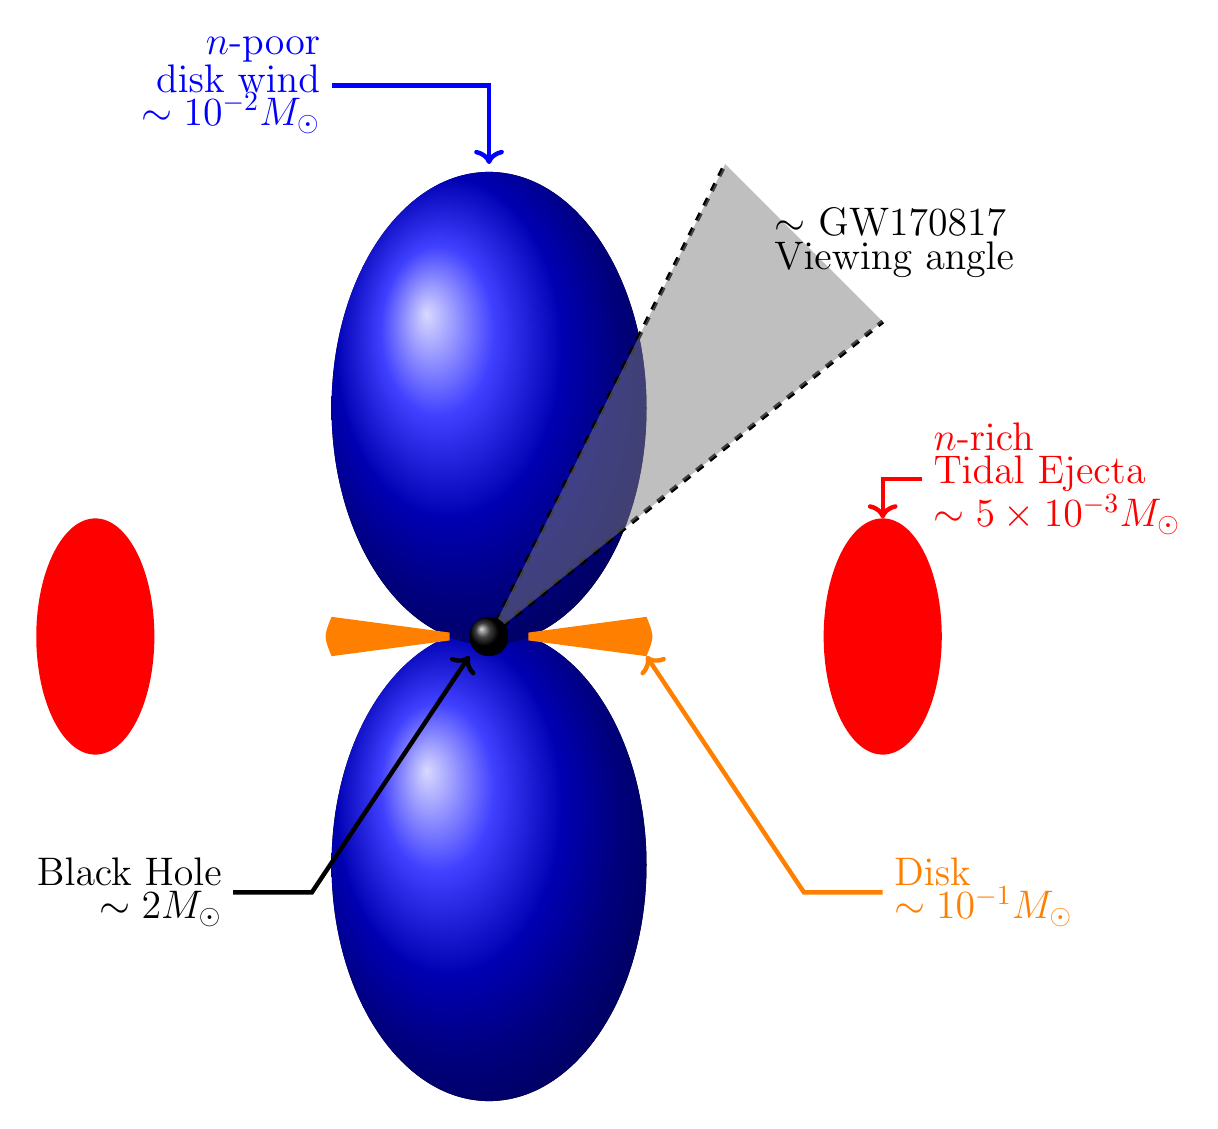
\begin{tikzpicture}
            \coordinate (origin) at (0,0);
            \pgfmathsetmacro{\dbx}{0.5}
            \pgfmathsetmacro{\dby}{0.05}
            \pgfmathsetmacro{\dex}{2.}
            \pgfmathsetmacro{\dey}{0.25}
            \pgfmathsetmacro{\dcc}{2.1}
            \pgfmathsetmacro{\tcx}{5.0}

            \foreach \i in {-1,1}
            {
              \fill[ball color=blue] (0, \i*2.9) ellipse (2 and 3);
            }

            \foreach \i in {-1,1}
            {
              % disk
              \fill[color=orange]
              (\i*\dbx,\dby) -- (\i*\dex,\dey)
              .. controls (\i*\dcc,0) .. (\i*\dex,-\dey)
              -- (\i*\dbx,-\dby) -- cycle;

              % tidal ejecta
              \fill[color=red] (\i*\tcx,0) ellipse (0.75 and 1.5);
            }

            % viewing
            \draw[dashed,ultra thick,black] (origin) -- (5,4);
            \draw[dashed,ultra thick,black] (origin) -- (3,6);
            \fill[color=gray,opacity=0.5] (origin) -- (5,4) -- (3,6) -- cycle;
            \node[right,align=left] at (3.5,5)
            {\Large $\sim$ GW170817\\ \Large Viewing angle};

            % bh
            \shade[ball color=black] (origin) circle (0.25);

            % text
            \draw[<-,red, ultra thick] (\tcx,1.5)
            -- ++(0.,0.5) -- ++(0.5,0)
            node[right,align=left]
            {\Large \color{red}$n$-rich\\\Large Tidal Ejecta\\ \Large $\sim 5\times 10^{-3}M_{\odot}$};

            \draw[<-,blue, ultra thick] (0,6) -- ++(0,1) -- ++(-2,0)
            node[left,align=right]
            {\Large \color{blue}$n$-poor\\\Large disk wind\\\Large $\sim 10^{-2}M_{\odot}$};

            \draw[<-,orange, ultra thick] (\dex,-\dey)
            -- ++(2,-3) -- ++(1,0)
            node[right,align=left]
            {\Large \color{orange}Disk\\\Large $\sim 10^{-1}M_{\odot}$};

            \draw[<-,black, ultra thick] (-0.25,-0.25)
            -- ++(-2,-3) -- ++(-1,0)
            node[left,align=right]
            {\Large \color{black}Black Hole\\ \Large $\sim 2 M_{\odot}$};
          \end{tikzpicture}
        }
      \end{center}
    \end{column}
  \end{columns}
  \begin{tiny}
    Co-design summer school, 2016
  \end{tiny}
\end{frame}

\begin{frame}
  \frametitle{Opacity}
  %\setlength{\unitlength}{1cm}
  \resizebox{12cm}{!}{
    \begin{tikzpicture}
      \node[inner sep=0pt] (rp) at (0,0)
      {\includegraphics[width=10cm]{skynet_ye_0p13/frame_0108}};
      \draw[ultra thick,red,<-] (1.5,-2) -- (2,-2.85)
      -- (2.25, -2.85) node[right] {\tiny Opaque to visible light};
      \draw[ultra thick,red,<-] (0.85,-2) -- (0.5,-2.85)
      -- (0.25,-2.85) node[left] {\tiny Not opaque};
    \end{tikzpicture}
  }
\end{frame}

\begin{frame}
  \frametitle{The Kilonova}
  \begin{center}
    \includegraphics[width=10cm]{swope-image}
  \end{center}
  M2H/UC Santa Cruz and Carnegie Observatories/Ryan Foley
\end{frame}

\begin{frame}
  \frametitle{Lets Focus on the Disk}
  \begin{center}
    \resizebox{12.cm}{!}{
      \begin{tikzpicture}
        \filldraw[black] (0,0) rectangle ++(12,8);
        % \node[right,align=left] at (0,0.25){\color{red}\textbf{JMM}+, in prep.};
        \node[inner sep=0pt] (wind) at (3,4)
        {\includegraphics[width=0.5\textwidth]{wind-3d-render}};
        \node[inner sep=0pt,rectangle,blue,ultra thick] (disk) at (9,5)
        {\includegraphics[width=0.4\textwidth]{disk_image_no_text}};
        \draw[blue,ultra thick] (6.5,3.5) rectangle ++(5,3.);
        \draw[blue,ultra thick] (3,4) -- (6.5,6.5);
        \draw[blue,ultra thick] (3,4) -- (6.5,3.5);
      \end{tikzpicture}
      %\includegraphics[width=7cm]{disk_3d_render}
      }
  \end{center}
\end{frame}

\begin{frame}
  \frametitle{Enter the Neutrino}
  \begin{columns}
    \begin{column}{6cm}
      \begin{center}
        \includegraphics[height=0.7\textheight]{gargamelle}\\
        CERN/Gargamelle
      \end{center}
    \end{column}
    \begin{column}{6cm}
      \begin{center}
        \includegraphics[width=\columnwidth]{neutrinos-fermilab}\\
        Fermilab
      \end{center}
    \end{column}
  \end{columns}
\end{frame}

\begin{frame}
  \frametitle{Neutrinos are required for nuclear reactions}
  \begin{center}
    \includegraphics[height=0.7\textheight]{Beta-minus_Decay}
  \end{center}
  Wikimedia Commons
\end{frame}

\begin{frame}
  \frametitle{Neutrino Transport Matters!}
  \begin{center}
    \includegraphics[height=0.8\textheight]{leptoneq/frame_0001}
    % \animategraphics[height=0.8\textheight,every=5,autoplay,loop,controls]
    % {5}{leptoneq/frame_}{0001}{0101}
  \end{center}
  \begin{tiny}
    \textbf{JMM}, B. R. Ryan, J. C. Dolence. ApJS \textbf{241} 30 (2019) 
  \end{tiny}
\end{frame}

\begin{frame}
  \frametitle{How Much Does Transport Matter?}
  \resizebox{12cm}{!}{
    \begin{tikzpicture}
      \coordinate (origin) at (0,0);

      \draw[blue] (origin) -- (5,3);

      \node[left] (tau1) at (0,2) {$\tau=1$};
      \draw[dashed,gray] (tau1) -- ++(5.5,0);

      \node[below] (m1) at (10./3.,0) {$10^0$};
      \draw[dashed,gray] (m1) -- ++(0,3.75)
      node[above] {\color{black}$10^{-1}$};
      
      \coordinate(tau2) at (0,1);
      \draw[dashed,gray] (tau2) -- ++(5,0);

      \node[below](m2) at (5./3.,0) {$10^{-1}$};
      \draw[dashed, gray] (m2) -- ++(0, 3.75)
      node[above] {\color{black}$10^{-2}$};

      \node[left] at (origin) {$\tau\ll 1$};
      \draw[ultra thick, black,->] (origin)
      -- ++(5, 0) node[below] {$\dot{M} (M_\odot/s)$};
      \draw[ultra thick, black, ->] (origin)
      -- ++(0, 3) node[left] {$\tau_\nu$};
      \draw[ultra thick, black, ->] (0,3.5)
      -- ++(5,0) node[above] {$M_d (M_\odot)$};

      \draw[<-,visible on=<1-2>] (5.2,3) -- ++(0.25,0) node[right,align=left]
      {\footnotesize \color{red}stay tuned};
      \node[inner sep=0pt,right, visible on=<3>] at (5,3) {\includegraphics[width=1cm]{curtis-pic}};
      \draw[<-,visible on=<1>] (5.2,2) -- ++(0.25,0) node[right,align=left]
      {\footnotesize abs. matters};
      \draw[<-,visible on=<2->] (5.2,2) -- ++(0.25,0) node[right,align=left]
      {\footnotesize $\sim 10^{-3}\dot{M}_{\text{ed}}$};

      \draw[<-] (5.2,1) -- ++(0.25,0) node[right,align=left]
      {\footnotesize emiss. doms.};

      \draw[<-] (0,-0.2) -- ++(0,-0.25) node[below,align=center]
      {\footnotesize no ignition};
    \end{tikzpicture}
    }
\end{frame}

\begin{frame}
  \frametitle{Ingredients In Kilonova Disk Modeling}
  \begin{itemize}
  \item General relativity
    \begin{itemize}
    \item Rotating black hole spacetime
    \end{itemize}
  \item Plasma physics
    \begin{itemize}
    \item Ideal magnetohydrodynamics
    \end{itemize}
  \item Nuclear physics
    \begin{itemize}
    \item Hot gas treated as being in nuclear-statistical equilibrium via \textbf{equation of state}
    \item Cooling outflow treated in postprocessing via \textbf{nuclear reaction networks}
    \end{itemize}
  \item Radiation physics
    \begin{itemize}
    \item Material is opaque to photons, can be incorporated in plasma physics
    \item Material \textit{not} opaque to \textbf{neutrinos}.
    \item Neutrinos can \textit{change the composition of the
        material} by converting neutrons to protons and vice versa.
    \end{itemize}
  \end{itemize}
\end{frame}

\begin{frame}
  \frametitle{Ingredients in Kilonova Disk Modeling}
  \begin{itemize}
  \item Mass conservation:
    \begin{small}
      \begin{displaymath}
        \partial_t \paren{{\color{red}\detg}\rho_0 u^t}
        + \partial_i\paren{{\color{red}\detg}\rho_0u^i} = 0
      \end{displaymath}
    \end{small}
  \item Momentum and Internal Energy Conservation:
    \begin{small}
      \begin{displaymath}
        \partial_t\sqrbrace{{\color{red}\detg} \paren{T^t_{\ \nu} + \rho_0u^t \delta^t_\nu}}
        + \partial_i\sqrbrace{{\color{red}\detg}\paren{T^i_{\ \nu} + \rho_0 u^i \delta^t_\nu}}
        = {\color{red}\detg} \paren{T^\kappa_{\ \lambda} {\color{red}\Gamma^\lambda_{\nu\kappa}} + {\color{blue}G_\nu}}
      \end{displaymath}
    \end{small}
  \item Magnetic Fields
    \begin{small}
      \begin{displaymath}
        \partial_t \paren{{\color{red}\detg} B^i}
        - \partial_j \sqrbrace{{\color{red}\detg}\paren{b^ju^i - b^i u^j}}
        = 0
      \end{displaymath}
    \end{small}
  \item Composition
    \begin{small}
      \begin{displaymath}
        \partial_t\paren{{\color{red}\detg}\rho_0 Y_e u^t}
        + \partial_i\paren{{\color{red}\detg}\rho_0Y_eu^i}
        = {\color{red}\detg} {\color{blue}G_{\text{ye}}}
      \end{displaymath}
    \end{small}
  \item Neutrino Transport
    \begin{small}
      \begin{displaymath}
        {\color{red}\frac{D}{d\lambda}}\paren{\frac{h^3\Inuf}{\eepsilon^3}}
        = \paren{\frac{h^2{\color{blue}\etanuf}}{\eepsilon^2}}
        - \paren{\frac{\eepsilon {\color{blue}\chinuf}}{h}} \paren{\frac{h^3\Inuf}{\eepsilon^3}},
      \end{displaymath}
    \end{small}
  \end{itemize}
\end{frame}

\begin{frame}
  \frametitle{Presenting $\nu\texttt{bhlight}$! \url{github.com/lanl/nubhlight}}
  \begin{center}
    \includegraphics[height=\textheight]{nubhlight-github}
  \end{center}
\end{frame}

\begin{frame}
  \frametitle{The August 2017 Disk (Miller et al., 2019)}
  \begin{center}
    \includegraphics[height=0.475\textheight]{gw170817disk_Ye_close/frame_0831} \\
    \includegraphics[height=0.475\textheight]{gw170817disk_Ye_far/frame_0831} 
    % \animategraphics[height=0.475\textheight,every=5,autoplay,loop,controls=off]
    % {10}{gw170817disk_Ye_close/frame_}{0001}{0837} \\
    % \animategraphics[height=0.475\textheight,every=5,autoplay,loop,controls=off]
    % {10}{gw170817disk_Ye_far/frame_}{0001}{0837} 
  \end{center}
  %\textbf{JMM}+, in prep.
\end{frame}

% \begin{frame}
%   \frametitle{Diversity in Outflows (Curtis et al. In Prep.)}
%   \begin{center}
%     \includegraphics[height=0.5\textheight]{sanjana_bhns_ye_combined}\\
%     \includegraphics[height=0.4\textheight]{sanjana_bhns_traced_comp}
%   \end{center}
% \end{frame}

% \begin{frame}
%   \frametitle{Diversity in Yields (Miller et al., 2019, Curtis et al.)}
%   \begin{center}
%     \resizebox{12cm}{!}{
%       \begin{tikzpicture}
%         \draw[ultra thick, black, ->] (-1,0) -- (6,0);
%         \node[above] at (5.5,0) {$\log_{10}M_d$};
%         \node[inner sep=0pt] at (0,-1.5) {\includegraphics[width=3cm]{collapsar/yields}};
%         \node[inner sep=0pt] at (4,-1.5) {
%           \includegraphics[width=3cm,clip,trim={0cm 0cm 1cm 1cm}]{sanjana_disk_yields_pt42}
%         };
%         \node[inner sep=0pt] at (2.,1.5) {
%           \includegraphics[width=3cm,clip,trim={0cm 0cm 1cm 1cm}]{sanjana_disk_yields_pt082}
%         };
%         \node[below] at (0,0)  {\tiny 2\% $M_\odot^*, Y_e=0.5$};
%         \node[above] at (2.,0) {\tiny 8\% $M_\odot$};
%         \node[below] at (4.,0) {\tiny 40\% $M_\odot$};
%         \draw[blue, thick, <-] (2.5,1.25)
%         -- ++(0.5,-0.5)
%         -- ++(0.5,0) node[right] {\tiny \color{blue}polar outflow};
%         \draw[red, thick, <-] (2.85,1.5) -- ++(1,0)
%         node[right]{\tiny\color{red}equatorial outflow};
%         \draw[black, thick, <-] (2.75,1.9) -- ++(1,0)
%         node[right]{\tiny total outflow};
%         \draw[deepgreen,thick,<-] (1.05,2.4) -- ++(-0.5,0)
%         node[left]{\tiny\color{deepgreen}solar abundance};
%       \end{tikzpicture}
%     }
%   \end{center}
% \end{frame}

\begin{frame}
  \frametitle{Neutrino Transport (Miller et al., 2019)}
  \begin{center}
    \includegraphics[width=0.9\textwidth]{nphys_frames/frame_00531}
    % \animategraphics[width=0.9\textwidth,every=10,autoplay,loop,controls=off]
    % {20}{nphys_frames/frame_}{00001}{00965}
  \end{center}
  \begin{tiny}
    \textbf{JMM} et al. PRD \textbf{100} 023008 (2019)
  \end{tiny}
\end{frame}

\begin{frame}
  \frametitle{Outflows, Nucleosynthesis, Observables}
  \begin{center}
    \resizebox{12cm}{!}{
      \begin{tikzpicture}
        \node[inner sep=0pt] at (6,6) {
          \includegraphics[width=5.5cm]{gw170817-yields-2}
        };
        \node[inner sep=0pt] at (0,4) {
          \includegraphics[height=0.9\textheight]{gw170817-ye-vs-theta-folded-5}
        };
        \node[inner sep=0pt] at (6,2) {
          \includegraphics[width=5.5cm]{spectral_evolution}
        };
        \node at (0,0) {\tiny \textbf{JMM} et al. PRD \textbf{100} 023008 (2019)};

        \node[align=center,fill=blue,visible on=<2->] at (3, 4)
        {\Huge \color{red}\textbf{This Story Changes}\\
          \Huge \color{red}\textbf{With Accretion Rate!}};
        \node[inner sep=0pt,visible on=<2->] at (1,1)
        {\includegraphics[width=2cm]{de-pic}};
        \node[inner sep=0pt,visible on=<2->] at (6,6)
        {\includegraphics[width=2cm]{curtis-pic}};
      \end{tikzpicture}
    }
  \end{center}
\end{frame}

% \begin{frame}
%   \frametitle{Electron Fraction}
%   \setlength{\unitlength}{1cm}
%   \begin{picture}(12,8)
%     \visible<1>{
%       \put(2,1){
%         \includegraphics[width=8cm]{gw170817-log-divergence-dyedt-tavg-wb}
%       }
%     }
%     \visible<2->{
%       \put(6,4){
%         \includegraphics[height=4cm]{gw170817-log-divergence-dyedt-tavg-wb}
%       }
%       \put(0,0.5){
%         \includegraphics[height=0.9\textheight]{gw170817-ye-vs-theta-folded-5}
%       }
%     }
%     \visible<3->{
%       \put(6,0.5){
%         \includegraphics[width=5.5cm]{gw170817-yields-2}
%       }
%     }
%     \visible<1->{
%       \put(0,0){
%         \begin{tiny}
%           \textbf{JMM} et al. PRD \textbf{100} 023008 (2019)
%         \end{tiny}
%       }
%     }
%   \end{picture}
% \end{frame}

% \begin{frame}
%   \frametitle{Light Curves}
%   \begin{center}
%     \includegraphics[width=0.9\columnwidth]{spectral_evolution}
%   \end{center}
%   \begin{tiny}
%     \textbf{JMM} et al. PRD \textbf{100} 023008 (2019)
%   \end{tiny}
% \end{frame}

\begin{frame}
  \frametitle{Accretion disks in supernovae?}
  \begin{columns}
    \begin{column}{6cm}
      \begin{center}
        \includegraphics[width=\columnwidth]{beppo-sax-light-curve}
      \end{center}
      Ruffini et al. BepoSAX telescope. arXiv:0705.2456
    \end{column}
    \begin{column}{6cm}
      \begin{center}
        \includegraphics[width=\columnwidth]{2250px-SN_1998bw}\\
        European Southern Observatory
      \end{center}
    \end{column}
  \end{columns}
\end{frame}

\begin{frame}
  \frametitle{Collapsars: Failed Supernovae}
  \begin{columns}
    \begin{column}{5cm}
      \begin{itemize}
      \item Accretion times $t\sim 10s$
      \item $\dot{M}$ between
        \begin{itemize}
        \item $10^{-4} M_\odot/s$
        \item $10^{-1} M_\odot/s$ 
        \end{itemize}
      \item $\rho \sim 10^{10}$ g$/$cm$^3$
      \end{itemize}
      \resizebox{\columnwidth}{!}{
        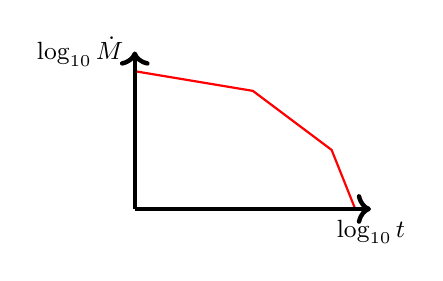
\begin{tikzpicture}
          \draw[thick,red]
          (0,1.75) -- (1.5,1.5) -- (2.5,0.75) -- (2.8,0);

          \coordinate (origin) at (0,0);
          \draw[ultra thick,->]
          (origin) -- ++(3,0)
          node[below] {\small $\log_{10}t$};
          \draw[ultra thick,->]
          (origin) -- ++(0,2)
          node[left] {\small $\log_{10}\dot{M}$};
        \end{tikzpicture}
      }
      \begin{tiny}
        Siegel, Barnes, Metzger. Nature \textbf{241} (2019)
      \end{tiny}
    \end{column}
    \begin{column}{7cm}
      \resizebox{\columnwidth}{!}{
        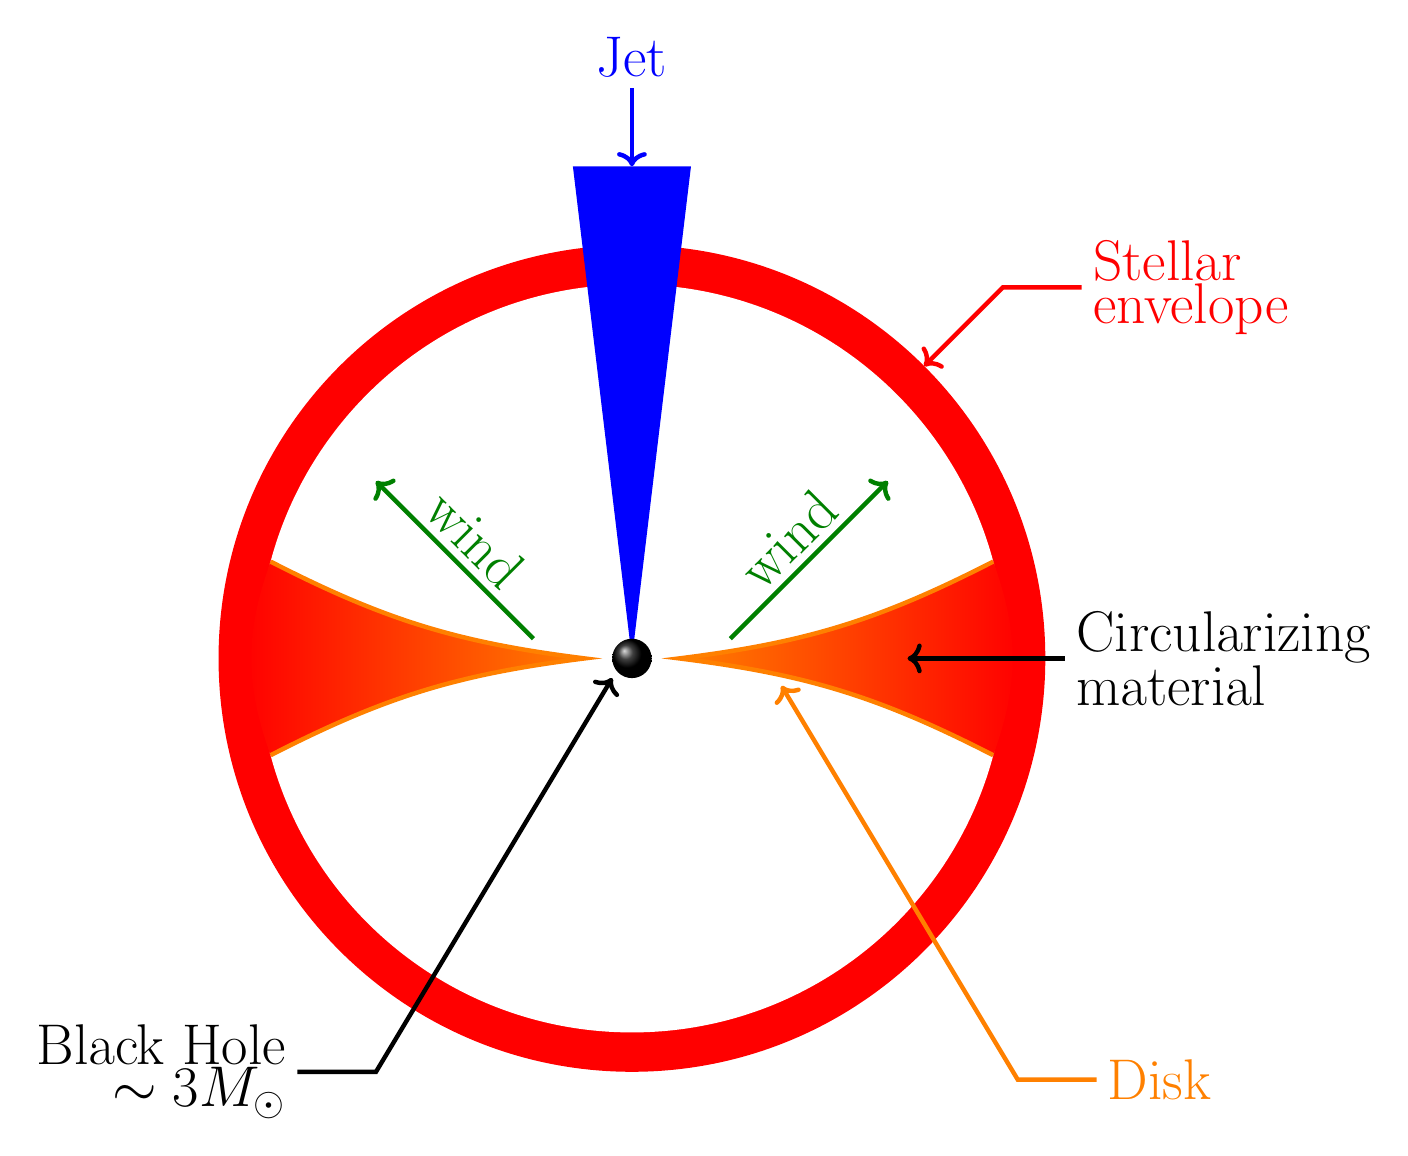
\begin{tikzpicture}
          \coordinate (origin) at (0,0);
          \pgfmathsetmacro{\pi}{3.14159}
          \pgfmathsetmacro{\dbx}{0.5}
          \pgfmathsetmacro{\dby}{0.05}
          \pgfmathsetmacro{\dex}{2.}
          \pgfmathsetmacro{\dey}{0.25}
          \pgfmathsetmacro{\dcc}{2.1}
          \pgfmathsetmacro{\tcx}{5.0}
          \pgfmathsetmacro{\rstar}{5}
          \pgfmathsetmacro{\wstar}{0.25}
          \pgfmathsetmacro{\wjet}{0.75}
          \pgfmathsetmacro{\tangle}{{45}}
          \pgfmathsetmacro{\tsx}{{(\rstar+\wstar)*cos(\tangle)}}
          \pgfmathsetmacro{\tsy}{{(\rstar+\wstar)*sin(\tangle)}}

          \pgfmathsetmacro{\cangle}{15}
          \pgfmathsetmacro{\cx}{(\rstar-\wstar)*cos(\cangle)}
          \pgfmathsetmacro{\cy}{(\rstar-\wstar)*sin(\cangle)}
          % \pgfmathsetmacro{\cend}{\dex + 0.1}
          \pgfmathsetmacro{\cend}{\dbx + 0.1}

          \newcommand{\msize}{\huge}

          % star
          \fill [color=red] (origin) circle (\rstar+\wstar);
          \fill [color=white] (origin) circle (\rstar-\wstar);

          % circularization
          \fill[color=red,
          left color=orange,
          middle color=orange,
          right color=red]
          (\cx,\cy) to [bend left=10] (\cend,0)
          to [bend left=10] (\cx,-\cy)
          to [bend right=20] cycle;
          
          \draw[orange,ultra thick]
          (\cx,\cy) to [bend left=10] (\cend, 0)
          to [bend left=10] (\cx,-\cy);

          \fill[color=red,
          right color=orange,
          middle color=orange,
          left color=red]
          (-\cx,\cy) to [bend right=10] (-\cend,0)
          to [bend right=10] (-\cx,-\cy)
          to [bend left=20] cycle;
          
          \draw[orange,ultra thick]
          (-\cx,\cy) to [bend right=10] (-\cend, 0)
          to [bend right=10] (-\cx,-\cy);

          % \foreach \i in {-1,1}
          % {
          %   % disk
          %   \fill[color=orange]
          %   (\i*\dbx,\dby) -- (\i*\dex,\dey)
          %   .. controls (\i*\dcc,0) .. (\i*\dex,-\dey)
          %   -- (\i*\dbx,-\dby) -- cycle;
          % }
          
          % jet
          \fill[color=blue] (origin) -- (-\wjet,1.25*\rstar) -- ++(2*\wjet,0) -- cycle;

          % bh
          \shade[ball color=black] (origin) circle (0.25);

          % wind
          \draw[deepgreen,ultra thick, ->]
          ({0.5*(\dbx + \dex)},\dey) -- ++(2,2);
          \draw ({0.5*(\dbx + \dex) + 1},{(\dey+1)})
          node[above,align=center,rotate=45]
          {\color{deepgreen}\msize wind};
          \draw[deepgreen,ultra thick, ->]
          ({-0.5*(\dbx + \dex)},\dey) -- ++(-2,2);
          \draw ({-(0.5*(\dbx + \dex) + 1)},{(\dey+1)})
          node[above,align=center,rotate=-45]
          {\color{deepgreen}\msize wind};          

          % text
          \draw[<-,orange, ultra thick] (\dex-0.1,-\dey-0.1)
          -- ++(3,-5) -- ++(1,0)
          node[right,align=left]
          {\msize \color{orange}Disk};
          
          \draw[<-,black, ultra thick] (-0.25,-0.25)
          -- ++(-3,-5) -- ++(-1,0)
          node[left,align=right]
          {\msize \color{black}Black Hole\\ \msize $\sim 3 M_{\odot}$};
          
          \draw[<-,red,ultra thick] (\tsx,\tsy)
          -- ++(1,1) -- ++(1,0)
          node[right,align=left]
          {\msize \color{red} Stellar\\ \msize envelope};

          \draw[<-,blue,ultra thick] (0, 1.25*\rstar) -- ++(0,1)
          node[above,align=center] {\msize \color{blue} Jet};

          \draw[<-,black,ultra thick]
          ({0.5*(\dex+\rstar)},0) -- ++(2,0) node[right,align=left]
          {\msize Circularizing\\ \msize material};
          
          \let\msize\undefined
        \end{tikzpicture}
      }
    \end{column}
  \end{columns}
\end{frame}

\begin{frame}
  \frametitle{Neutrinos matter differently for collapsars!}
  \resizebox{12cm}{!}{
    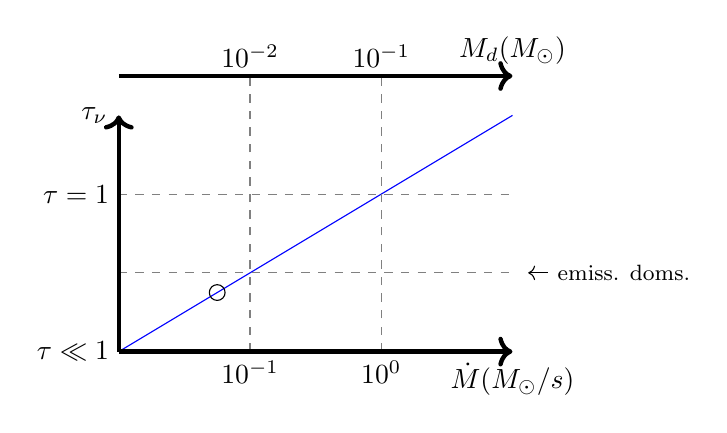
\begin{tikzpicture}
      \coordinate (origin) at (0,0);

      \draw[blue] (origin) -- (5,3);

      \node[left] (tau1) at (0,2) {$\tau=1$};
      \draw[dashed,gray] (tau1) -- ++(5.5,0);

      \node[below] (m1) at (10./3.,0) {$10^0$};
      \draw[dashed,gray] (m1) -- ++(0,3.75)
      node[above] {\color{black}$10^{-1}$};
      
      \coordinate(tau2) at (0,1);
      \draw[dashed,gray] (tau2) -- ++(5,0);

      \node[below](m2) at (5./3.,0) {$10^{-1}$};
      \draw[dashed, gray] (m2) -- ++(0, 3.75)
      node[above] {\color{black}$10^{-2}$};

      \node[left] at (origin) {$\tau\ll 1$};
      \draw[ultra thick, black,->] (origin)
      -- ++(5, 0) node[below] {$\dot{M} (M_\odot/s)$};
      \draw[ultra thick, black, ->] (origin)
      -- ++(0, 3) node[left] {$\tau_\nu$};
      \draw[ultra thick, black, ->] (0,3.5)
      -- ++(5,0) node[above] {$M_d (M_\odot)$};

      \draw[<-] (5.2,1) -- ++(0.25,0) node[right,align=left]
      {\footnotesize emiss. doms.};

      \draw (5./4.,3./4.) circle (0.1);
    \end{tikzpicture}
    }
\end{frame}

\begin{frame}
  \frametitle{Building a Collapsar Disk}
  \begin{center}
    \includegraphics[height=0.45\textheight]{collapsar/close/anim_RHO/frame_0001}
  \end{center}
  \begin{center}
    \includegraphics[height=0.45\textheight]{collapsar/close/anim_Ye/frame_0001}
  \end{center}
\end{frame}

\begin{frame}
  \frametitle{Building a Collapsar Disk}
  \begin{center}
    \includegraphics[height=0.45\textheight]{collapsar/close/anim_RHO/frame_0240}
    % \animategraphics[height=0.45\textheight,every=7,autoplay,loop,controls]
    % {3}{collapsar/close/anim_RHO/frame_}{0001}{0240}
  \end{center}
  \begin{center}
    \includegraphics[height=0.45\textheight]{collapsar/close/anim_Ye/frame_0240}
    % \animategraphics[height=0.45\textheight,every=7,autoplay,loop,controls]
    % {3}{collapsar/close/anim_Ye/frame_}{0001}{0240}
  \end{center}
\end{frame}

\begin{frame}
  \frametitle{Outflow Properties}
  \begin{columns}
    \begin{column}{5cm}
      \begin{center}
        \includegraphics[height=0.9\textheight]{collapsar/ye_v_theta}
      \end{center}
    \end{column}
    \begin{column}{7cm}
      \begin{center}
        \includegraphics[height=0.9\textheight]{collapsar/s-and-vr-v-theta}
      \end{center}
    \end{column}
  \end{columns}
\end{frame}

\begin{frame}
  \frametitle{Electron Fraction and Nucleosynthesis}
  \begin{columns}
    \begin{column}{5cm}
      \begin{center}
        \includegraphics[height=0.9\textheight]{collapsar/ye_v_theta}
      \end{center}
    \end{column}
    \begin{column}{7cm}
      \begin{center}
        \includegraphics[width=\columnwidth]{collapsar/yields}
      \end{center}
      \begin{tiny}
        Miller et al., ApJ \textbf{902}, 66 (2020)
      \end{tiny}
    \end{column}
  \end{columns}
\end{frame}

\begin{frame}
  \frametitle{Limits of the Setup}
  \begin{columns}
    \begin{column}{6cm}
      \begin{center}
        \includegraphics[width=\columnwidth]{collapsar/rhovr}
      \end{center}
    \end{column}
    \begin{column}{6cm}
      \begin{center}
        \includegraphics[width=\columnwidth]{collapsar/binding_energy}
      \end{center}
    \end{column}
  \end{columns}
  \begin{tiny}
    Miller et al., ApJ \textbf{902}, 66 (2020)
  \end{tiny}
\end{frame}

\begin{frame}
  \frametitle{Lots of fun science!}
  \setlength{\unitlength}{1cm}
  \begin{picture}(12,8)
      \put(0,1) {
        \includegraphics[width=0.5\textwidth]{collapsar/ye_statistics}
      }
      \put(6,4) {
        \includegraphics[width=0.5\textwidth]{collapsar/rho_Ye_snap_t5000}
      }
      \put(5,0.0) {
        \includegraphics[width=0.6\textwidth]{collapsar/selected_traces_lattitude_cut}
      }
      \put(0,0){
        {\footnotesize Miller et al., ApJ \textbf{902}, 66 (2020)}
      }
  \end{picture}
\end{frame}

\begin{frame}
  \frametitle{Conclusions}
  \begin{columns}
    \begin{column}{7cm}
      \begin{itemize}
      \item The heaviest elements in the universe produced in some
        crazy cool systems!
      \item Need GRRMHD and neutrino transport!
      \item NS Mergers:
        \begin{itemize}
        \item Likely source of heavy elements in our
          universe
        \item Disks can produce blue component of kilonova
        \end{itemize}
      \item Large diversity in outflows and disk physics
        \begin{itemize}
        \item Angular structure in the outflow is generic.
        \item Set by balance between MHD turbulence and neutrino physics
        \end{itemize}
      \end{itemize}
    \end{column}
    \begin{column}{5cm}
      \includegraphics[width=\columnwidth,clip,trim={150 0 150 0}]{3d_render}
    \end{column}
  \end{columns}
\end{frame}

\backupbegin

\begin{frame}
  \frametitle{Accretion Rates}
  \begin{center}
    \includegraphics[width=0.9\textwidth]{mdot_edd}
  \end{center}
\end{frame}

\begin{frame}
  \frametitle{Accretion Rates}
  \begin{center}
    \includegraphics[width=0.9\textwidth]{mdot_edd_nu}
  \end{center}
\end{frame}

\begin{frame}
  \frametitle{Presenting $\nu\texttt{bhlight}$!}
  \begin{itemize}
  \item General relativistic radiation magnetohydrodynamics for kilonova disks
  \item \textbf{Magnetized gas} via \textit{finite volume methods}
    \begin{itemize}
    \item Standard second-order Gudonov scheme
    \item Cell-centered constrained transport for magnetic fields
    \item WENO5 reconstruction
    \item Local Lax-Friedrichs Riemann solver
    \end{itemize}
  \item \textbf{Neutrinos} via \textit{Monte Carlo methods}
    \begin{itemize}
    \item Explicit integration along geodesics
    \item Probabilistic emissivity, absorption, and scattering
    \item Novel biasing scheme ensures all processes well-sampled
    \end{itemize}
  \item \textbf{Coupled} via \textit{operator splitting}
  \item Built on top of $\texttt{HARM}$, $\texttt{grmonty}$, and
    $\texttt{bhlight}$.
  \end{itemize}
\end{frame}

% \begin{frame}
%   \frametitle{A Growing Suite of Models}
%   \begin{columns}
%     \begin{column}{5cm}
%       \begin{center}
%         \includegraphics[width=\columnwidth]{disks_run_MMa_3d_scatter}
%       \end{center}
%     \end{column}
%     \begin{column}{7cm}
%       \resizebox{\columnwidth}{!}{
%         \begin{tikzpicture}
%           \coordinate (origin) at (0,0);
%           \pgfmathsetmacro{\pi}{3.14159}
%           \pgfmathsetmacro{\dbx}{0.5}
%           \pgfmathsetmacro{\dby}{0.05}
%           \pgfmathsetmacro{\dex}{2.}
%           \pgfmathsetmacro{\dey}{0.25}
%           \pgfmathsetmacro{\dcc}{2.1}
%           \pgfmathsetmacro{\tcx}{5.0}
%           \pgfmathsetmacro{\rstar}{5}
%           \pgfmathsetmacro{\wstar}{0.25}
%           \pgfmathsetmacro{\wjet}{0.75}
%           \pgfmathsetmacro{\tangle}{{45}}
%           \pgfmathsetmacro{\tsx}{{(\rstar+\wstar)*cos(\tangle)}}
%           \pgfmathsetmacro{\tsy}{{(\rstar+\wstar)*sin(\tangle)}}
% 
%           \pgfmathsetmacro{\cangle}{15}
%           \pgfmathsetmacro{\cx}{(\rstar-\wstar)*cos(\cangle)}
%           \pgfmathsetmacro{\cy}{(\rstar-\wstar)*sin(\cangle)}
%           % \pgfmathsetmacro{\cend}{\dex + 0.1}
%           \pgfmathsetmacro{\cend}{\dbx + 0.1}
% 
%           \newcommand{\msize}{\huge}
% 
%           % star
%           \fill [color=red] (origin) circle (\rstar+\wstar);
%           \fill [color=white] (origin) circle (\rstar-\wstar);
% 
%           % circularization
%           \fill[color=red,
%           left color=orange,
%           middle color=orange,
%           right color=red]
%           (\cx,\cy) to [bend left=10] (\cend,0)
%           to [bend left=10] (\cx,-\cy)
%           to [bend right=20] cycle;
%           
%           \draw[orange,ultra thick]
%           (\cx,\cy) to [bend left=10] (\cend, 0)
%           to [bend left=10] (\cx,-\cy);
% 
%           \fill[color=red,
%           right color=orange,
%           middle color=orange,
%           left color=red]
%           (-\cx,\cy) to [bend right=10] (-\cend,0)
%           to [bend right=10] (-\cx,-\cy)
%           to [bend left=20] cycle;
%           
%           \draw[orange,ultra thick]
%           (-\cx,\cy) to [bend right=10] (-\cend, 0)
%           to [bend right=10] (-\cx,-\cy);
% 
%           % \foreach \i in {-1,1}
%           % {
%           %   % disk
%           %   \fill[color=orange]
%           %   (\i*\dbx,\dby) -- (\i*\dex,\dey)
%           %   .. controls (\i*\dcc,0) .. (\i*\dex,-\dey)
%           %   -- (\i*\dbx,-\dby) -- cycle;
%           % }
%           
%           % jet
%           \fill[color=blue] (origin) -- (-\wjet,1.25*\rstar) -- ++(2*\wjet,0) -- cycle;
% 
%           % bh
%           \shade[ball color=black] (origin) circle (0.25);
% 
%           % wind
%           \draw[deepgreen,ultra thick, ->]
%           ({0.5*(\dbx + \dex)},\dey) -- ++(2,2);
%           \draw ({0.5*(\dbx + \dex) + 1},{(\dey+1)})
%           node[above,align=center,rotate=45]
%           {\color{deepgreen}\msize wind};
%           \draw[deepgreen,ultra thick, ->]
%           ({-0.5*(\dbx + \dex)},\dey) -- ++(-2,2);
%           \draw ({-(0.5*(\dbx + \dex) + 1)},{(\dey+1)})
%           node[above,align=center,rotate=-45]
%           {\color{deepgreen}\msize wind};          
% 
%           % text
%           \draw[<-,orange, ultra thick] (\dex-0.1,-\dey-0.1)
%           -- ++(3,-5) -- ++(1,0)
%           node[right,align=left]
%           {\msize \color{orange}Disk};
%           
%           \draw[<-,black, ultra thick] (-0.25,-0.25)
%           -- ++(-3,-5) -- ++(-1,0)
%           node[left,align=right]
%           {\msize \color{black}Black Hole\\ \msize $\sim 3 M_{\odot}$};
%           
%           \draw[<-,red,ultra thick] (\tsx,\tsy)
%           -- ++(1,1) -- ++(1,0)
%           node[right,align=left]
%           {\msize \color{red} Stellar\\ \msize envelope};
% 
%           \draw[<-,blue,ultra thick] (0, 1.25*\rstar) -- ++(0,1)
%           node[above,align=center] {\msize \color{blue} Jet};
% 
%           \draw[<-,black,ultra thick]
%           ({0.5*(\dex+\rstar)},0) -- ++(2,0) node[right,align=left]
%           {\msize Circularizing\\ \msize material};
%           
%           \let\msize\undefined
%         \end{tikzpicture}
%       }
%     \end{column}
%   \end{columns}
% \end{frame}

% \begin{frame}
%   \frametitle{A Growing Suite of Models}
%   \begin{columns}
%     \begin{column}{4cm}
%       \begin{center}
%         \includegraphics[width=\columnwidth]{disks_run_MMa_3d_scatter}
%       \end{center}
%     \end{column}
%     \begin{column}{8cm}
%       \begin{center}
%         \includegraphics[width=\columnwidth]{disks_run_thermo_params}
%       \end{center}
%     \end{column}
%   \end{columns}
%   \begin{itemize}
%   \item Soon to be many more.
%   \item $\gtrapprox 50$ by the end of the DR
%   \end{itemize}
% \end{frame}

\begin{frame}
  \frametitle{Turbulence and $Y_e$}
  \resizebox{12cm}{!}{
    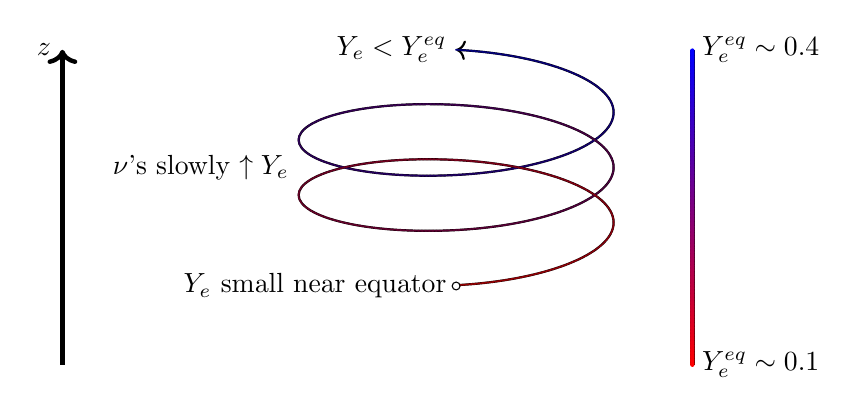
\begin{tikzpicture}
      \coordinate(origin) at (-2,0);

      \draw[ultra thick, black, ->] (origin) -- ++ (0, 4)
      node[left] {$z$};

      \draw[ultra thick,colormorph={0.8pt}{red}{blue}] (6,0) -- ++(0,4);
      \node[right] at (6,0) {$Y_e^{eq}\sim 0.1$};
      \node[right] at (6,4) {$Y_e^{eq}\sim 0.4$};

      \draw[thick,
      decoration={aspect=0.31,segment length=7mm,amplitude=2cm, coil},
      colormorph={0.4pt}{deepblue}{deepred},
      decorate,arrows={<[bend]-}] (3,4) -- (3,1);
      \node[draw,fill=white,circle,inner sep=1pt] at (3,1) {};
      \node[left] at (3,1) {$Y_e$ small near equator};
      \node[left] at (1.,2.5) {$\nu$'s slowly $\uparrow Y_e$};
      \node[left] at (3,4) {$Y_e < Y_e^{eq}$};
    \end{tikzpicture}
  }
\end{frame}

\begin{frame}
  \frametitle{$Y_e$ is set by the balance of Turbulence and
    Neutrinos!}
  \begin{center}
    \includegraphics[width=0.9\textwidth]{collapsar/ye_time_scales_t5000}
  \end{center}
  {\footnotesize Miller et al., ApJ \textbf{902}, 66 (2020)}
\end{frame}

\begin{frame}
  \frametitle{$Y_e$ is set by the balance of Turbulence and
    Neutrinos!}
  \begin{displaymath}
      Y_{\rm e}(z/H) = \braket{\text{min}(Y_{\rm e})}_{\text{trc}}
      + \braket{\frac{d Y_{\rm e}}{dt}}_{t,\text{trc}} \paren{H\braket{\frac{dz}{dt}}_{t,\text{trc}}^{-1}}\paren{\frac{z}{H} - \braket{\text{min}(z/H)}_{\text{trc}}}
    \end{displaymath}
    \begin{columns}
      \begin{column}{6cm}
        \includegraphics[width=\columnwidth]{collapsar/vertical-structure-params}
      \end{column}
      \begin{column}{6cm}
        \includegraphics[width=\columnwidth]{collapsar/model-vs-vertical-structure}
      \end{column}
    \end{columns}
    {\footnotesize Miller et al., ApJ \textbf{902}, 66 (2020)}
\end{frame}

\begin{frame}
  \frametitle{How Important is Absorption?}
  \begin{columns}
    \begin{column}{6cm}
      \begin{itemize}
      \item With no absorption:
      \end{itemize}
      \begin{center}
        \includegraphics[height=0.85\textheight]{collapsar/ye_em_v_theta}
      \end{center}
    \end{column}
    \begin{column}{6cm}
      \begin{itemize}
      \item Opacity suppresses change in $Y_e$
      \end{itemize}
      \begin{center}
        \includegraphics[width=\columnwidth]{collapsar/transient-dtau}
      \end{center}
      \begin{tiny}
        Miller et al., ApJ \textbf{902}, 66 (2020)
      \end{tiny}
    \end{column}
  \end{columns}
\end{frame}

\backupend

\end{document}